\documentclass[../main]{subfiles}

\begin{document}
\chapter{Fantastic SQUIDs}
\label{app:squid}

\lipsum[1-2]

\begin{figure}[h]
    \centering
    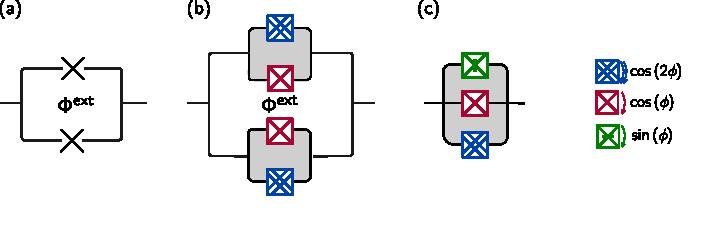
\includegraphics{appendix/img/squid.pdf}
    \caption{\textbf{SQUID made with nonsinusoidal Josephson junctions.}
    (a) SQUID made with nonsinusoidal Josephson junctions.
    (b) Circuit model with ideal Josephson elements (up to the second order). The gray area means that the total flux in the mesh is fixed to zero.
    (c) Circuit model of the effective Josephson potential at the two ends of the SQUID.
    }
    \label{fig:squid}
\end{figure}

\lipsum[3-7]


\end{document}
